\documentclass{article}
\usepackage[utf8]{inputenc}
\usepackage{graphicx}
\usepackage{mathtools} 
\usepackage{textcomp}
\usepackage{titling}
\usepackage{subfig}
\usepackage{amsmath}
\usepackage[parfill]{parskip}
\usepackage{xcolor}
\definecolor{LightGray}{gray}{0.9}
\usepackage{titlesec}
\setcounter{secnumdepth}{4}
\usepackage[a4paper,left=1cm,right=1cm,top=1cm,bottom=1.5cm,]{geometry}
\usepackage{eqparbox}
\usepackage{enumitem}
\usepackage{graphicx}
\newcommand*{\Scale}[2][4]{\scalebox{#1}{\ensuremath{#2}}}%
\usepackage{centernot}

\title{\vspace{-2cm} EE4218 L7 - Technology Mapping}
\date{\vspace{-5ex}}

\begin{document}
\maketitle

\section{General introduction}
Recall that after \textit{Architectural Synthesis}, we had \textit{Logic Synthesis}.

Logic synthesis consisted of the following sub-steps \dots
\begin{enumerate}[label*=\arabic*.]
    \item Logic Optimization
        \begin{enumerate}[label*=\arabic*.]
            \item Minimizing undesirable redundancies; Using K-Maps, boolean identities, etc...
        \end{enumerate}
    \item Technology Mapping (ie. Library Binding)
        \begin{enumerate}[label*=\arabic*.]
            \item Mapping logic to library cells
            \item The 'binding' that is going on here is of a \textbf{microscopic} level, in contrast to the \textbf{macroscopic} 'binding' that happened during architectural synthesis
        \end{enumerate}
\end{enumerate}

We will focus on Technology Mapping now.

\section{Introduction to Technology Mapping}
Maps the technology \textbf{independent} network resulting from logic optimization,
to logic cells that are available in a technology \textbf{dependent} cell library

Whilst performing technology mapping, we utilize algorithms to furthur minimize area while still meeting constraints (eg. timing constraints).

\subsection{Types of technology mapping}
Broadly speaking, it depends on whether we are developig for ASICs or FPGAs.

\begin{itemize}
    \item ASICs
        \begin{itemize}
            \item Usually library cells are more primitive than that of FPGAs
            \item Limited set of pre-designed cells
        \end{itemize}
    \item FPGAs
        \begin{itemize}
            \item LUT-based (Xilinx): Each FPGA cell is termed a \textit{Configurable Logic Block}
            \item MUX-based (Actel): Each FPGA cell consists of a number of multiplexers
        \end{itemize}
\end{itemize}

\subsubsection{(ASIC) cell library}
As an example, the IBM standard-cell library used for the POWER4 is as follows

\begin{figure}[htp]
    \centering
    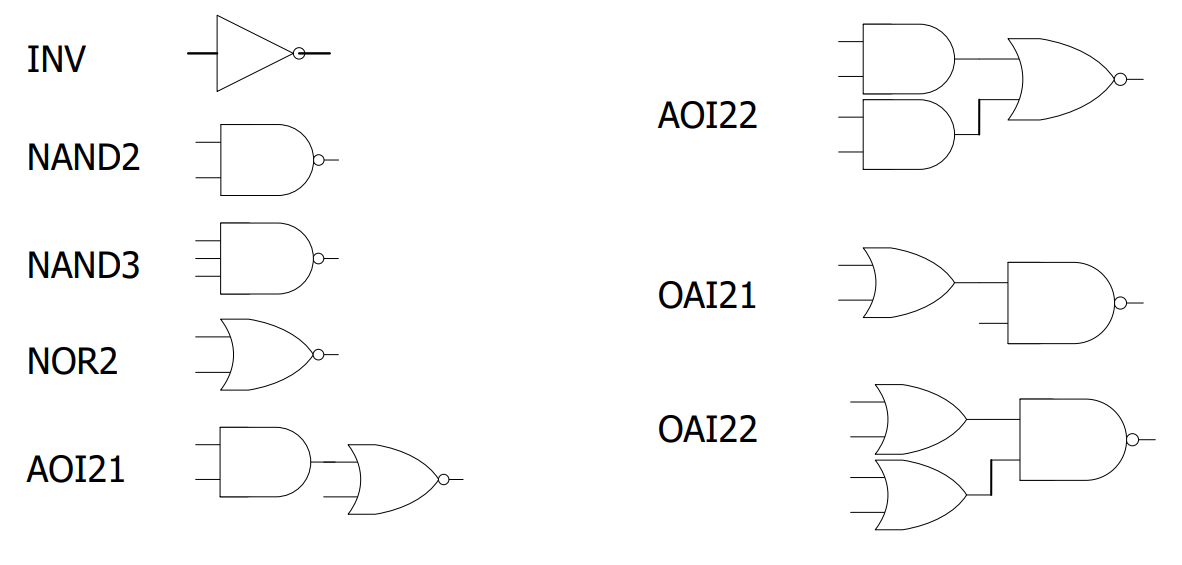
\includegraphics[width=12cm, scale=1]{S2/asicCellLibrary.PNG}
    \caption{Designer has the following cells to build upon}
\end{figure}

\newpage
\subsubsection{(FPGA) LUT-based cells}

\paragraph{Multiplexer}\mbox{}\\
Let's begin with a \textit{4-1} MUX.
\begin{figure}[htp]
    \centering
    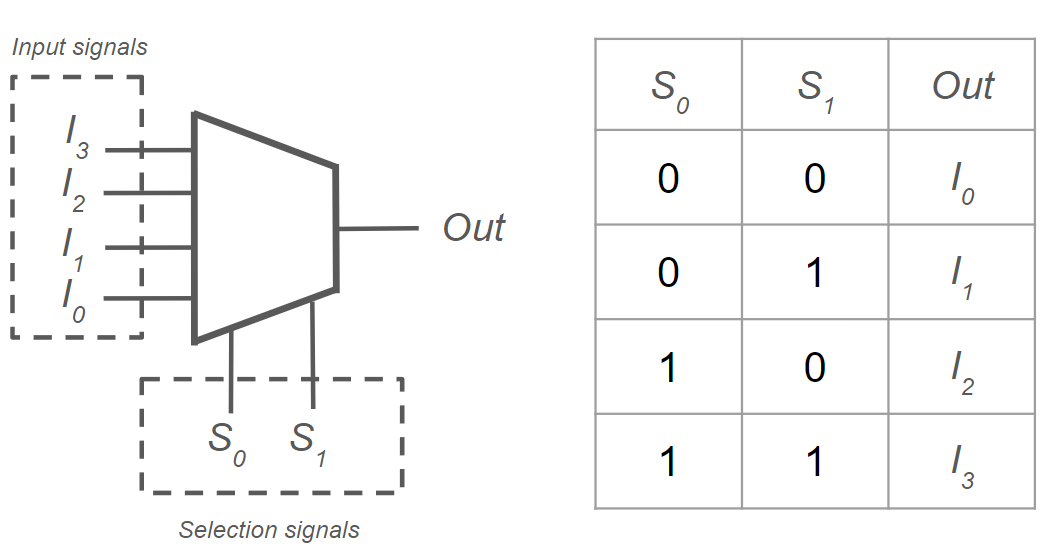
\includegraphics[width=8cm, scale=1]{S2/4-1_mux.PNG}
    \caption{\textit{4-1} MUX, with associated truth table}
\end{figure}

\begin{itemize}
    \item In a \textit{4-1} MUX, we have 2 \textit{selection} signals which select amongst $2^{2}$ \textit{input} signals.
    \item Note that \textbf{each} of the $\{I_{0},I_{1},I_{2},I_{3}\}$ signals could be 0 or 1, therefore this \textit{4-1} MUX has $2^{2^{num\_input\_signals}} = 16$ possible \textbf{input-output} combinations.
    \item Recognize that a \textit{logic function} is a \textit{mapping} from input to output (singular in this case), hence we could represent 16 different combinational functions this way.
    \item Herein is the underlying logic behind an LUT - if we can configure the value of these input signals, then we can construct 16 different combinational functions.
\end{itemize}

\paragraph{Constructing an LUT}\mbox{}\\
Using the ideas above, the \textit{4-1} MUX above can thus be converted into a 2LUT (2-input LUT)

\begin{minipage}[t]{0.5\textwidth}
    \centering
    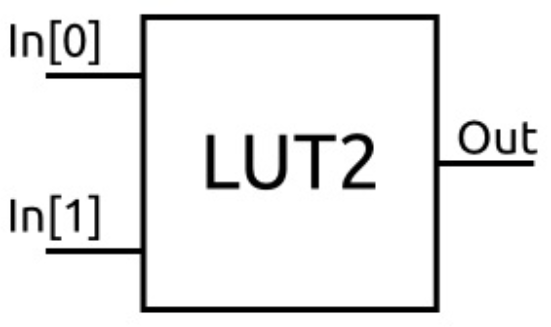
\includegraphics[width=6cm, scale=1]{S2/2LUT.PNG}
    \captionof{figure}{2LUT\\
                        \textit{Selection signals} are our \textit{input addresses}}
\end{minipage}%
\begin{minipage}[t]{0.5\textwidth}
    \centering
    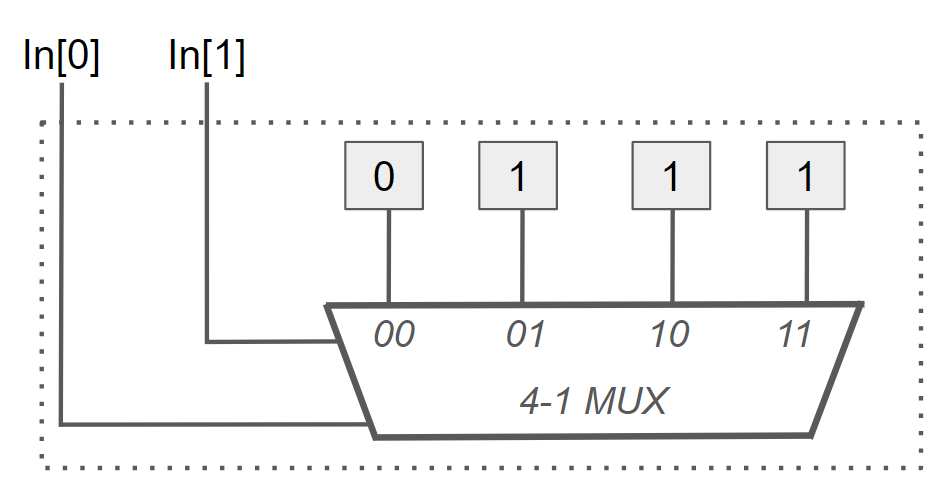
\includegraphics[width=6cm, scale=1]{S2/2LUT_muxView.PNG}
    \captionof{figure}{\textbf{0110} represents the \textbf{output} of a particular truth table (ie. combinational function) that this 2LUT implements}
\end{minipage}%


\begin{itemize}
    \item The LUT consists of a block of SRAM that is indexed by the LUT's inputs
    \item Output of the LUT is whatever value is in the indexed location in it's SRAM
\end{itemize}

\vspace{0.25cm}
Let's examine the internals of the LUT.

\begin{itemize}
    \item LUT is built out of \dots
        \begin{enumerate}
            \item SRAM bits to hold some configurable memory (\textit{CRAM}), we term this the \textit{LUT-mask}
            \item Set of multiplexers to select the bit of CRAM that will be directed to output
        \end{enumerate}
    \item To implement a k-LUT (an LUT that can implement any k-input function), we require \dots
        \begin{enumerate}
            \item $2^{k}$ SRAM bits. Note that there are $2^{2^{k}}$ possible combinational functions, but we are setting the SRAM bits (ie. outputs) only for a \textbf{certain} combinational function we want to implement.
                    Therefore, since the combinational function has $k$ inputs, it should have $2^{k}$ possible outputs.
            \item $2^{k}:1$ MUX, to select the output for our \textbf{certain} combinational function
        \end{enumerate}
\end{itemize}

\begin{minipage}[t]{0.5\textwidth}
    \centering
    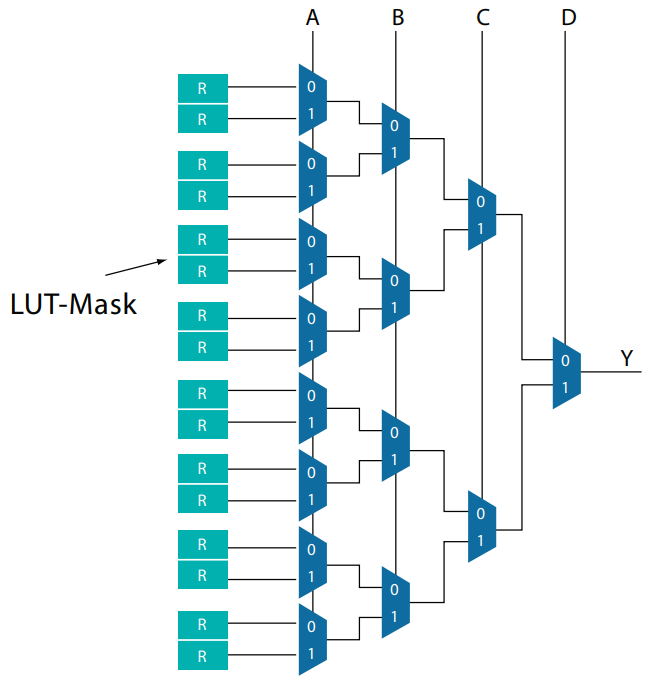
\includegraphics[width=9cm, scale=1]{S2/4LUT.PNG}
    \captionof{figure}{4LUT}
\end{minipage}%
\begin{minipage}[t]{0.5\textwidth}
    \centering
    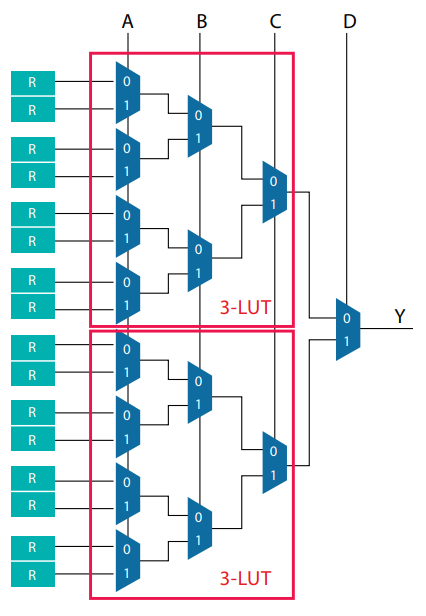
\includegraphics[width=7cm, scale=1]{S2/4LUT_3LUT.PNG}
    \captionof{figure}{4LUT implemented with two 3LUT and a 2:1 MUX}
\end{minipage}%

\paragraph{CLB}\mbox{}\\
Finally, we can understand how the CLB is built.

\begin{figure}[htp]
    \centering
    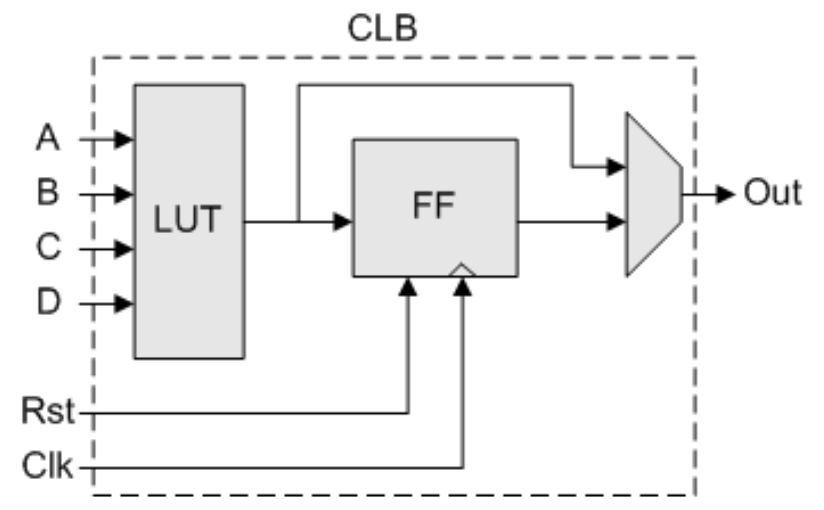
\includegraphics[width=10cm, scale=1]{S2/CLB.PNG}
    \caption{Configurable Logic Block}
\end{figure}


\subsubsection{(FPGA) MUX-based cells}

\paragraph{Tweaking the Multiplexer}\mbox{}\\
Remember the \textit{4-1} MUX earlier?

\begin{figure}[htp]
    \centering
    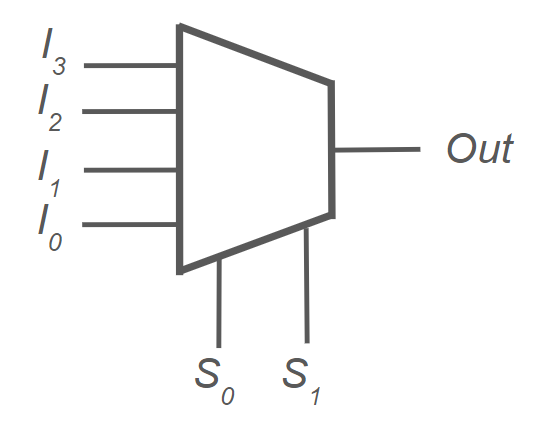
\includegraphics[width=5cm, scale=1]{S2/muxTweak.PNG}
    \caption{\textit{4-1} MUX}
\end{figure}

Previously, the \textit{4-1} MUX could only implement a 2-input combinational function (via $\{S_{0}, S_{1}\}$), since $\{I_{0},I_{1},I_{2},I_{3}\}$ were 'fixed' at binary values 0 or 1.
However, what if we allowed $\{I_{0},I_{1},I_{2},I_{3}\}$ to act as inputs as well? Then the \textit{4-1} MUX can implement up to a 6-input combinational function!


Hence, we can furthur expand on the truth table of the MUX.

\begin{minipage}[t]{0.5\textwidth}
    \centering
    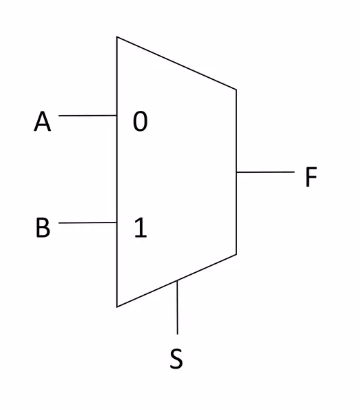
\includegraphics[width=4cm, scale=1]{S2/2-1_mux.PNG}
    \captionof{figure}{2-1 MUX}
\end{minipage}%
\begin{minipage}[t]{0.5\textwidth}
    \centering
    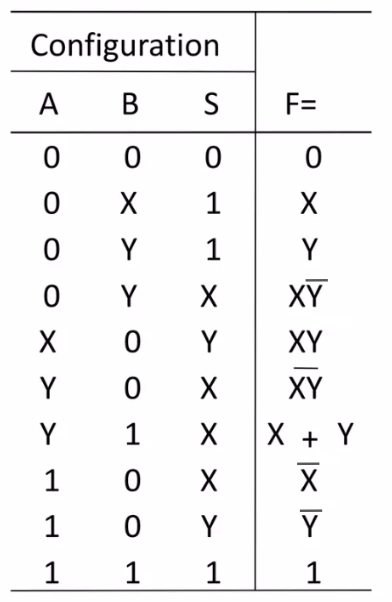
\includegraphics[width=4cm, scale=1]{S2/nonExTruthTable.PNG}
    \captionsetup{justification=centering}
    \captionof{figure}{Expanded truth table.\\
                        Note that it is non-exhaustive, since we expect there to be $3^{3}$ possible combinations}
\end{minipage}%

This new way of viewing MUXes will make sense soon.

\paragraph{Shannon's decomposition theorem}\mbox{}\\
Allows for any logic function to be expanded and broken down into parts.
This means that it is possible to implement any logical function using multiplexers.

\begin{figure}[htp]
    \centering
    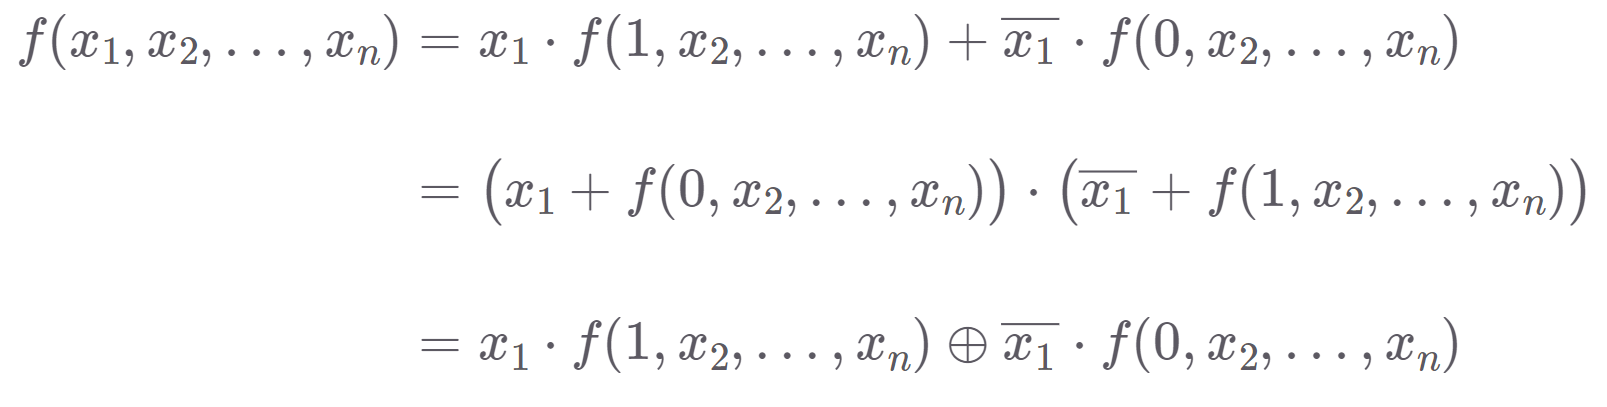
\includegraphics[width=10cm, scale=1]{S2/shannonExpansion.PNG}
    \caption{Shannon's decomposition theorem}
\end{figure}

Let's apply Shannon's decomposition theorem now.

\begin{enumerate}
    \item Suppose we have a function $F(a,b,c)$
    \item Expanding it using SDT, we get $\Scale[2]{F = a \cdot F_{a} + \bar{a} \cdot F_{\bar{a}}}$
    \item Therefore, $F$ can be implemented as a 2-1 MUX as seen below.
\end{enumerate}

\begin{figure}[htp]
    \centering
    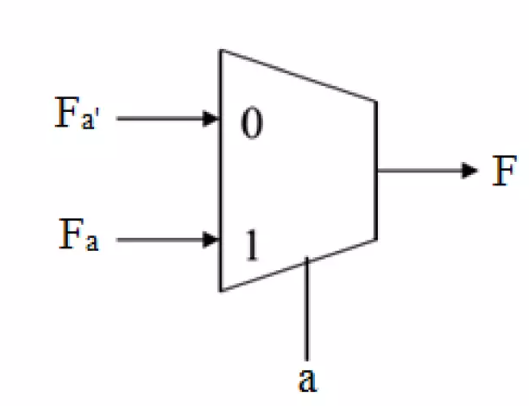
\includegraphics[width=6cm, scale=1]{S2/SDT_1.PNG}
    \caption{When $a=1, F_{a}$ is channeled to output\\
             When $a=0, F_{\bar{a}}$ is channeled to output}
\end{figure}

We can recursively apply SDT \dots
\begin{enumerate}[label*=\arabic*.]
    \item $\Scale[2]{F = a \cdot F_{a} + \bar{a} \cdot F_{\bar{a}}}$
        \begin{enumerate}[label*=\arabic*.]
            \item $\Scale[2]{F_{a} = b \cdot F_{ab} + \bar{b} \cdot F_{a\bar{b}}}$
            \item $\Scale[2]{F_{\bar{a}} = b \cdot F_{\bar{a}b} + \bar{b} \cdot F_{\bar{a}\bar{b}}}$
        \end{enumerate}
    \item $\Scale[2]{F = \{a \cdot (b \cdot F_{ab} + \bar{b} \cdot F_{a\bar{b}})\}
                        + \{\bar{a} \cdot (b \cdot F_{\bar{a}b} + \bar{b} \cdot F_{\bar{a}\bar{b}})\}}$
    \item $\Scale[2]{F = \{a \cdot b \cdot F_{ab} + a \cdot \bar{b} \cdot F_{a\bar{b}}\}
                        + \{\bar{a} \cdot b \cdot F_{\bar{a}b} + \bar{a} \cdot \bar{b} \cdot F_{\bar{a}\bar{b}}\}}$

\end{enumerate}

\begin{figure}[htp]
    \centering
    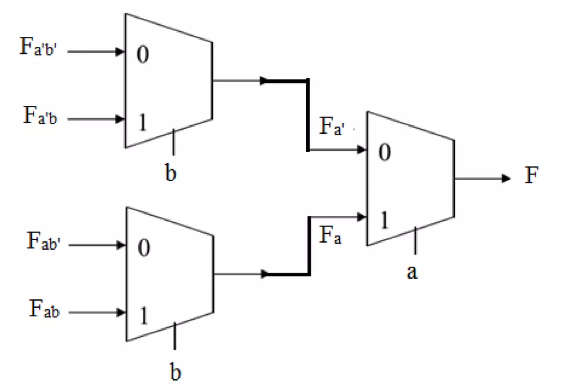
\includegraphics[width=9cm, scale=1]{S2/SDT_2.PNG}
    \caption{We see a 'tree' of MUXes forming...}
\end{figure}

\paragraph{Logic modules}\mbox{}\\
Actel uses the above MUXes to form MUX-based logic cells.

\begin{figure}[htp]
    \centering
    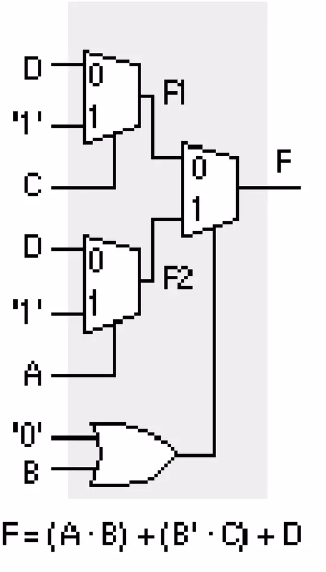
\includegraphics[width=5cm, scale=1]{S2/actel.PNG}
    \caption{Implementation of combinational logic, using what Actel terms \textit{ACT1 Logic Module}}
\end{figure}

\newpage
\subsection{Flow of Technology Mapping}
Technology Mapping can be broadly broken down into 3 steps \dots

\begin{enumerate}
    \item Decomposition
        \begin{itemize}
            \item Restructures the logic network \textbf{and library cells} using \textbf{base} primitives
            \item The purpose of this is so that \textit{pattern matching} at the later stage will be easier (since they are all expressed in terms of the same base primitives)
            \item Decomposition to base primitives decreases the level of optimization that can be done (tradeoff for increased simplicity)
        \end{itemize}
    \item Partitioning
        \begin{itemize}
            \item Partitions the large network into smaller sub-networks
            \item The purpose of this is so that the \textit{Matching and Covering} stage is easier to handle (ie. divide and conquer strategy)
            \item Partitioning introduces module boundaries, decreasing the level of optimization that can be done (tradeoff for increased simplicity)
        \end{itemize}
    \item Matching and Covering
        \begin{itemize}
            \item Determines which library cells may be used to implement a set of nodes in our logic network
        \end{itemize}
\end{enumerate}

\section{Logic Decomposition}
We decompose the logic network \textbf{and library cells} using a choice of base primitives, which creates a new representation.

Note that logic decomposition is a heuristic that does not provide unique solutions.

\begin{minipage}[t]{0.3\textwidth}
    \centering
    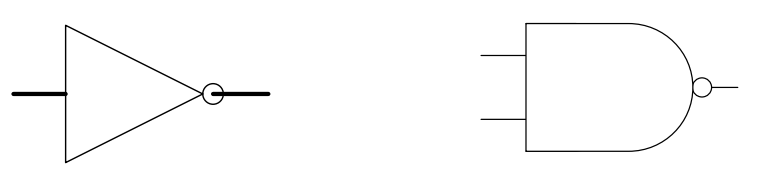
\includegraphics[width=6cm, scale=1]{S3/basePrimitives.PNG}
    \captionsetup{justification=centering}
    \captionof{figure}{\textit{NAND2} and \textit{INV} gates are popular choices for base primitives, since \textbf{every} boolean function can be implemented with a \textbf{combination} of them}
\end{minipage}%
\begin{minipage}[t]{0.7\textwidth}
    \centering
    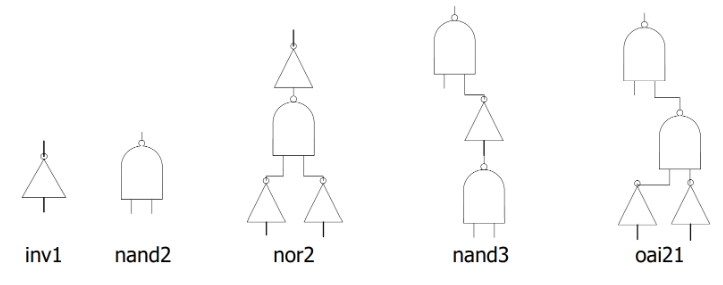
\includegraphics[width=12cm, scale=1]{S3/decomposedLibrary.PNG}
    \captionsetup{justification=centering}
    \captionof{figure}{Decomposed library cells (of the IBM POWER4).\\We term these \textit{Pattern Trees}}
\end{minipage}

\vspace{0.25cm}
Suppose we have a complex gate in our logic network, shown below.

\begin{figure}[htp]
    \centering
    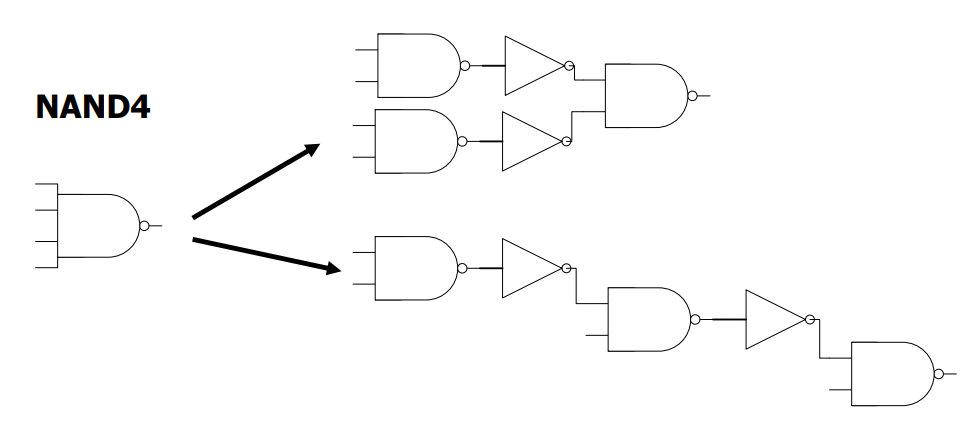
\includegraphics[width=11cm, scale=1]{S3/nand4_matching.PNG}
    \caption{\textit{NAND4} gate may be decomposed in two different ways}
\end{figure}

We note that the two decompositions are \textit{functionally} identically, but \textit{structurally} (and hence timing-wise) different.
Therefore, complex gates may be \textit{matched} by completely different patterns.

\section{Partioning}
\begin{itemize}
    \item Reduce a \textit{MIMO} (multi-input-multi-output) network into a collection of \textit{MISO} (multi-input-single-output) sub-networks,
            with each sub-network termed as a \textit{subject graph}
    \item This allows for a \textit{Divide and Conquer} approach to the \textit{Covering problem} that we will see later
\end{itemize}

\subsection{Partioning algorithm}
\begin{enumerate}
    \item Mark vertices with multiple-out degrees; Edges connected to these marked vertices define the partition boundary
    \item Partition accordingly to form \textit{subject graphs} (ie. break the circuit at fanout points)
    \item Note that we may furthur (recursively) partition the subject graphs
\end{enumerate}

\begin{figure}[htp]
    \centering
    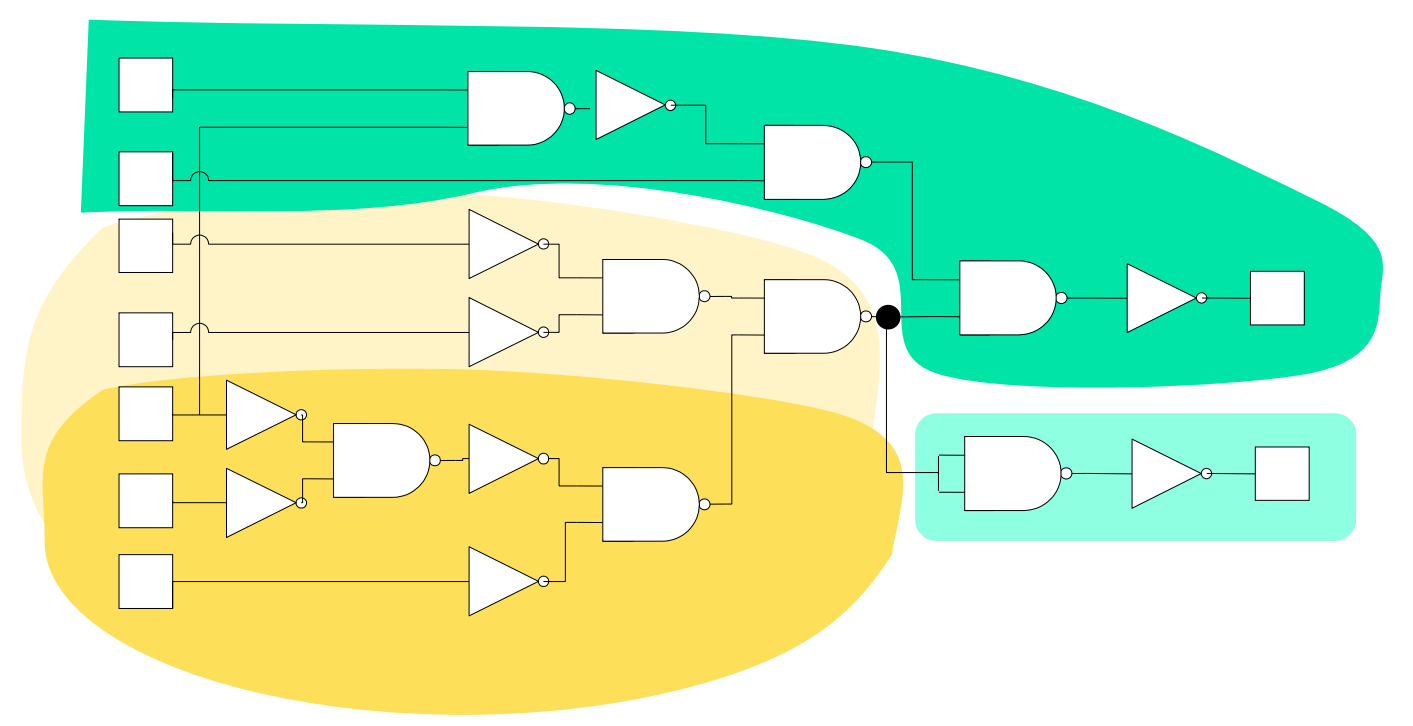
\includegraphics[width=12cm, scale=1]{S3/partitionedGraph.PNG}
    \caption{Partitioned graph}
\end{figure}

\section{Pattern Matching and Covering}
There are two main types of pattern matching \dots
\begin{itemize}
    \item Structural Matching
    \item Boolean Matching
\end{itemize}

\subsection{Structural Matching}
Intuitively, it is matching by looking at shapes.
We match the logic network with the library cells recursively, until the entire network is mapped.

\begin{minipage}[t]{0.5\textwidth}
    \centering
    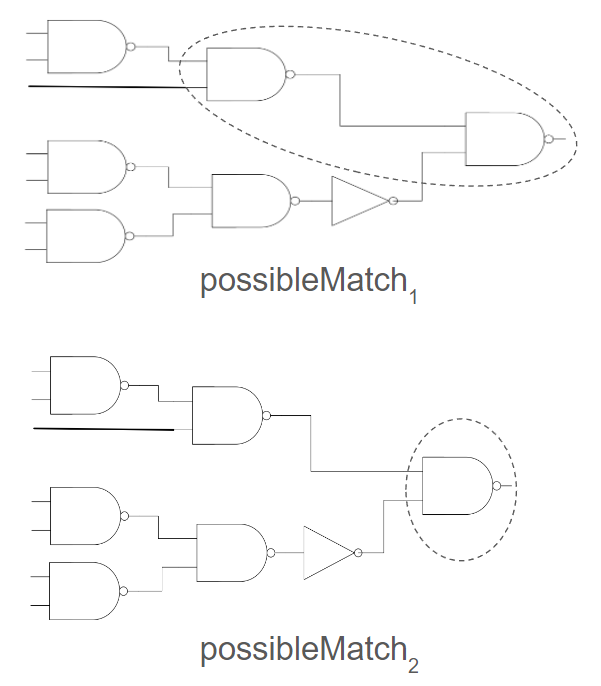
\includegraphics[width=6cm, scale=1]{S4/possibleMatches.PNG}
    \captionsetup{justification=centering}
    \captionof{figure}{Possible matches (depending on which library cell we map to)}
\end{minipage}%
\begin{minipage}[t]{0.5\textwidth}
    \centering
    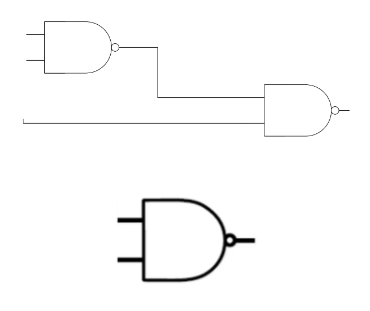
\includegraphics[width=6cm, scale=1]{S4/libraryCells.PNG}
    \captionsetup{justification=centering}
    \captionof{figure}{Library cells available}
\end{minipage}%

As seen in the example above, there may be multiple matches available for the same set of nodes. 
We need an algorithm to find which are the best matches that we eventually use to cover the entire network.

\subsubsection{Recursive algorithm for Structural Matching}
Recursive algorithm to identify if \textit{pattern tree} (decomposed library cells) is \textit{isomorphic} (ie. same shape) to a subgraph of the subject tree.
Note that it works only when \textbf{one} type of base primitive is used in the decomposition (furthur note: \textit{Inverter} can be seen as \textit{NAND} gate with inputs shorted).

\paragraph{Some definitions before we get started}\mbox{}\\
\begin{minipage}[t]{0.5\textwidth}
    \vspace{0pt}
    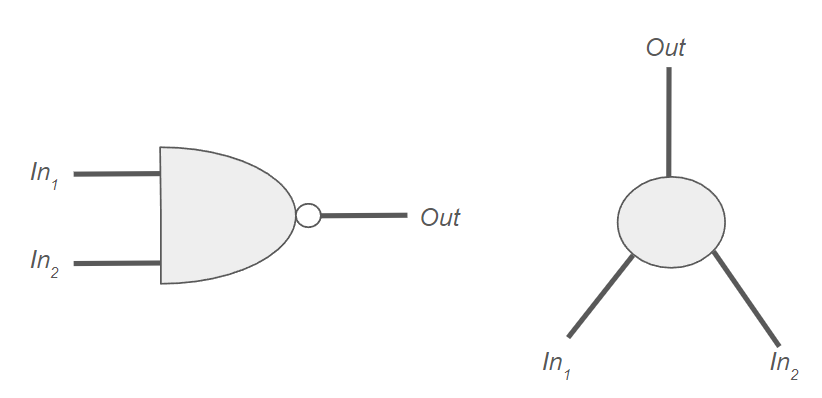
\includegraphics[width=9cm, scale=1]{S4/graphChildren.PNG}
    \captionof{figure}{Vertex with degree=2}
\end{minipage}%
\begin{minipage}[c]{0.5\textwidth}
    Note that orientation of the tree! \newline

    \begin{itemize}
        \item Degree of vertex used to indicate the number of children
        \item \textit{u} is the root of the \textbf{pattern} graph
        \item \textit{v} is a vertex of the \textbf{subject} graph
    \end{itemize}
\end{minipage}


\paragraph{Algorithm}\mbox{}\\
\begin{figure}[htp]
    \centering
    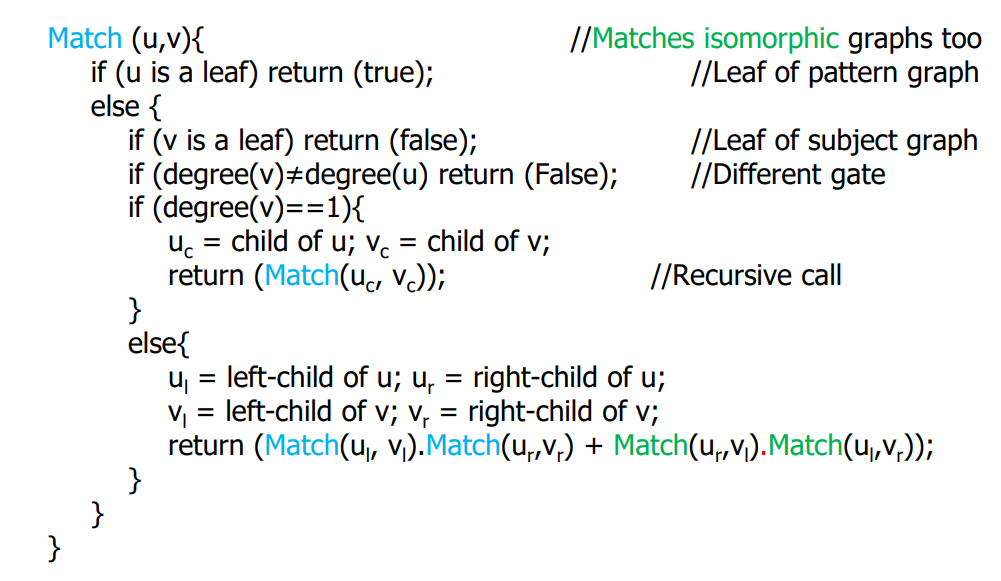
\includegraphics[width=12cm, scale=1]{S4/matchingAlgorithm.PNG}
    \caption{Recursive algorithm for matching}
\end{figure}

\paragraph{Algorithm - Example 1}\mbox{}\\

\begin{minipage}[t]{0.5\textwidth}
    \centering
    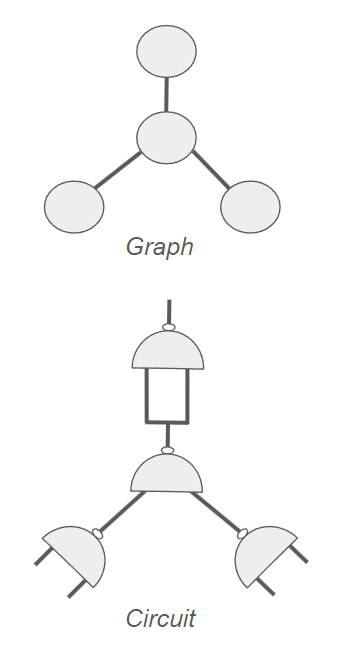
\includegraphics[width=3cm, scale=1]{S4/subjectGraph.PNG}
    \captionsetup{justification=centering}
    \captionof{figure}{Subject graph, with corresponding circuit}
\end{minipage}%
\begin{minipage}[t]{0.5\textwidth}
    \centering
    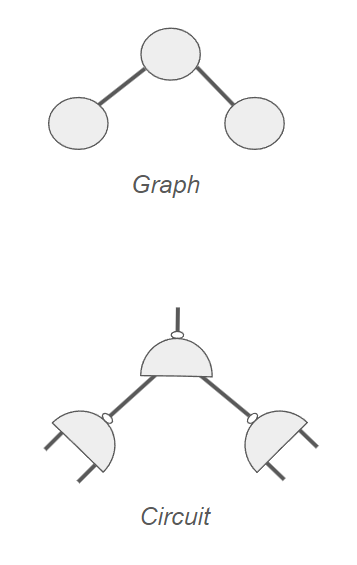
\includegraphics[width=3cm, scale=1]{S4/patternGraph.PNG}
    \captionsetup{justification=centering}
    \captionof{figure}{Pattern graph, with corresponding circuit}
\end{minipage}%

\newpage
\begin{minipage}[t]{0.6\textwidth}
    \vspace{0pt}
    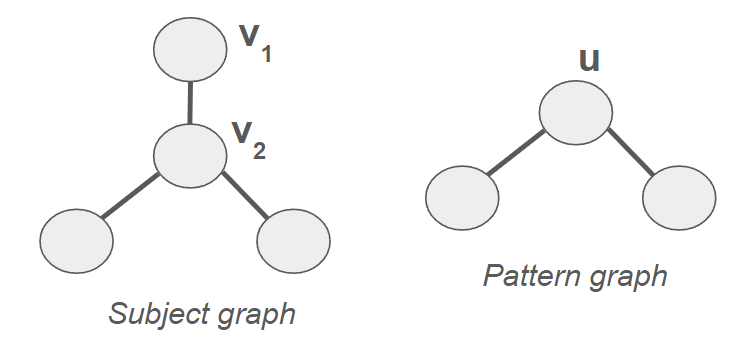
\includegraphics[width=12cm, scale=1]{S4/subjectPatternGraph.PNG}
\end{minipage}%
\begin{minipage}[t]{0.4\textwidth}
    \vspace{0pt}
    \begin{itemize}
        \item If we start from vertex $v_{1}$ of the subject graph, then we have that
                $degree(v_{1})=1 \neq degree(u)=2$. Thererfore no match.
        \vspace{0.25cm}
        \item If we start from vertex $v_{2}$ of the subject graph (assume that $v_{1}$ was matched by other library cells),
         then we have that $degree(v_{2})=2 = degree(u)=2$. Thererfore match \textit{might} be possible. We will enter the \textit{else} statement for furthur checks, eventually finding that match is possible.
    \end{itemize}
\end{minipage}

\vspace{2cm}
\paragraph{Algorithm - Example 2}\mbox{}\\
We need to find all possible patterns in the subject network first, before we can decide which combination of patterns is optimal.

\begin{figure}[htp]
    \centering
    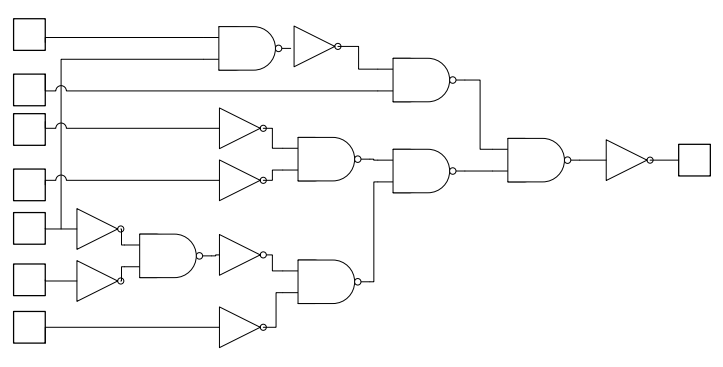
\includegraphics[width=13cm, scale=1]{S4/problemStatement.PNG}
    \caption{Subject network}
\end{figure}

\begin{figure}[htp]
    \centering
    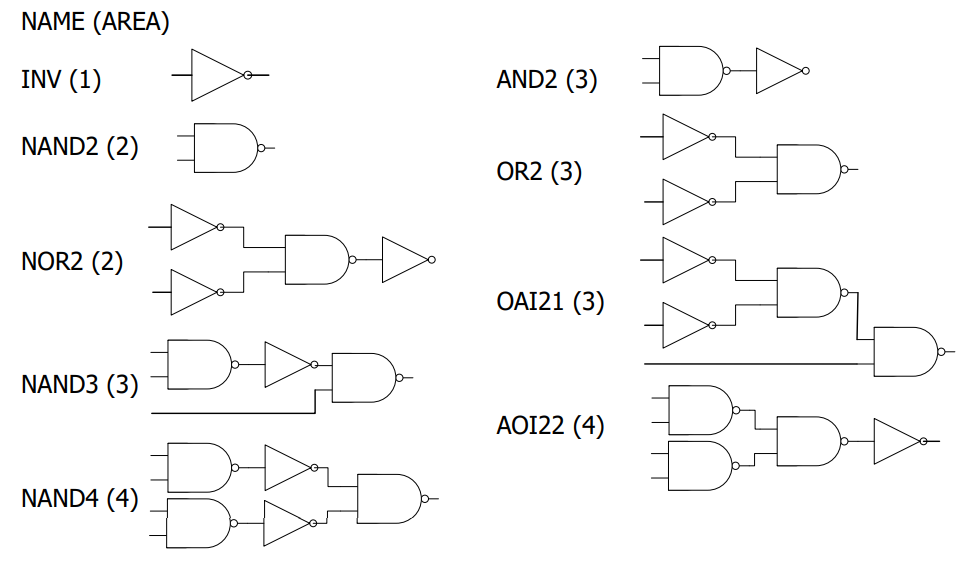
\includegraphics[width=13cm, scale=1]{S4/pattern_library.PNG}
    \caption{Cell Library}
\end{figure}

\begin{minipage}[t]{0.5\textwidth}
    \centering
    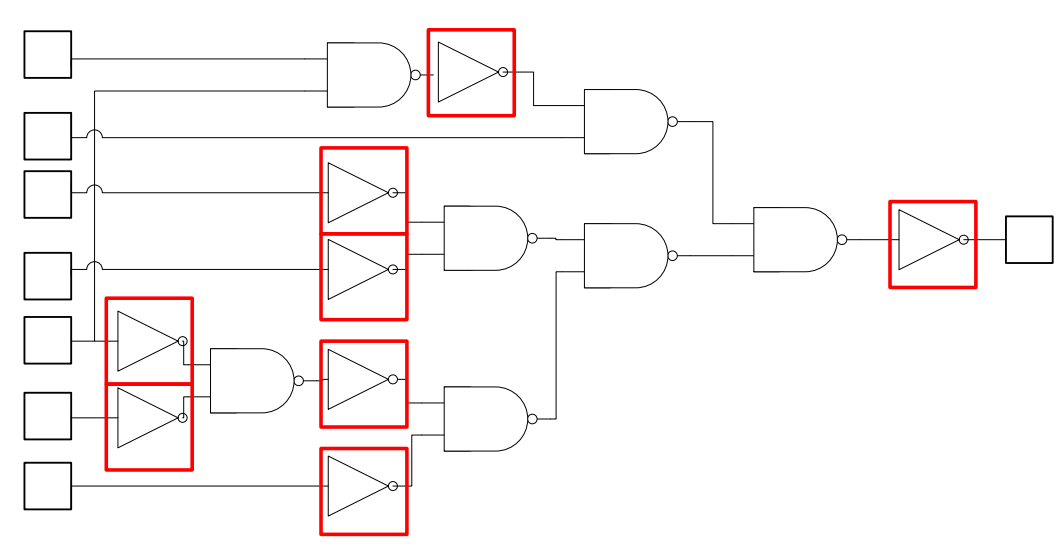
\includegraphics[width=9cm, scale=1]{S4/inv_pattern.PNG}
    \captionsetup{justification=centering}
    \captionof{figure}{\textit{INV} patterns}
\end{minipage}%
\begin{minipage}[t]{0.5\textwidth}
    \centering
    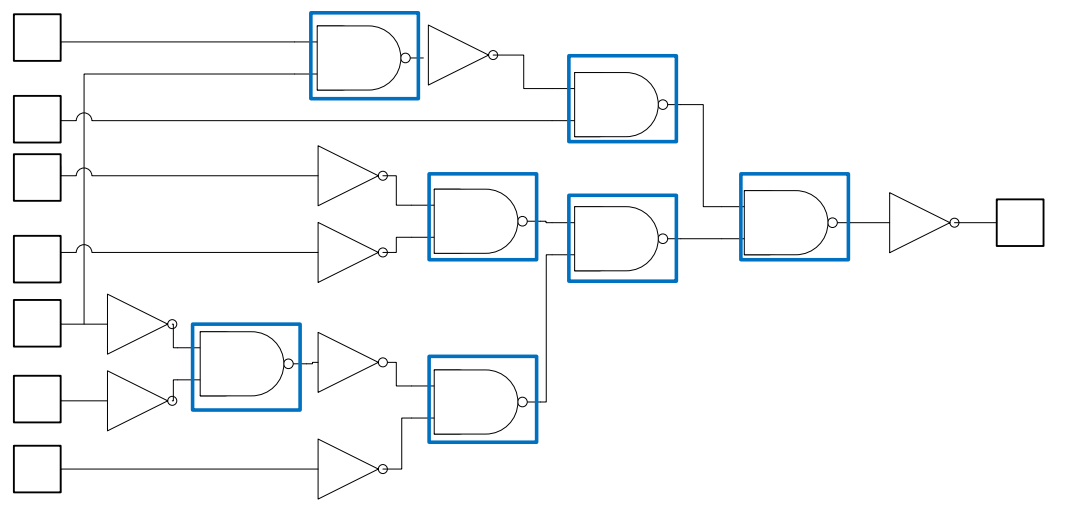
\includegraphics[width=9cm, scale=1]{S4/nand2_pattern.PNG}
    \captionsetup{justification=centering}
    \captionof{figure}{\textit{NAND2} patterns}
\end{minipage}%

\vspace{1cm}
\begin{minipage}[t]{0.5\textwidth}
    \centering
    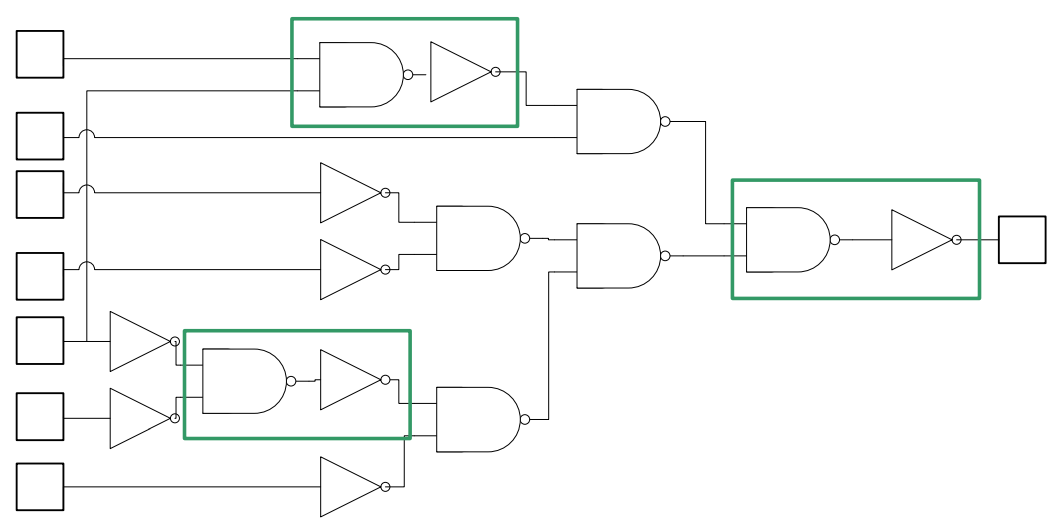
\includegraphics[width=9cm, scale=1]{S4/and2_pattern.PNG}
    \captionsetup{justification=centering}
    \captionof{figure}{\textit{AND2} patterns}
\end{minipage}%
\begin{minipage}[t]{0.5\textwidth}
    \centering
    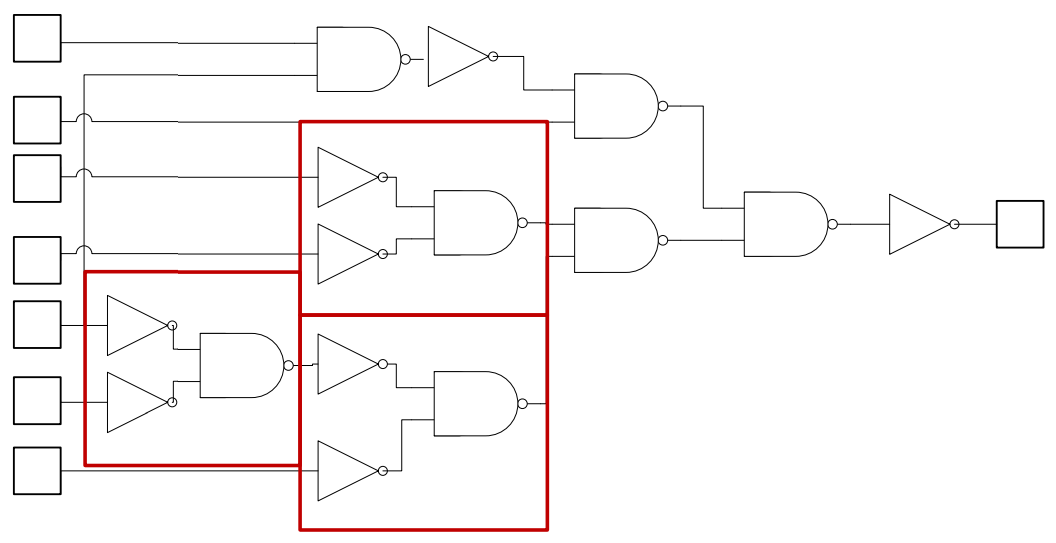
\includegraphics[width=9cm, scale=1]{S4/or2_pattern.PNG}
    \captionsetup{justification=centering}
    \captionof{figure}{\textit{OR2} patterns}
\end{minipage}%

\vspace{1cm}
\begin{minipage}[t]{0.5\textwidth}
    \centering
    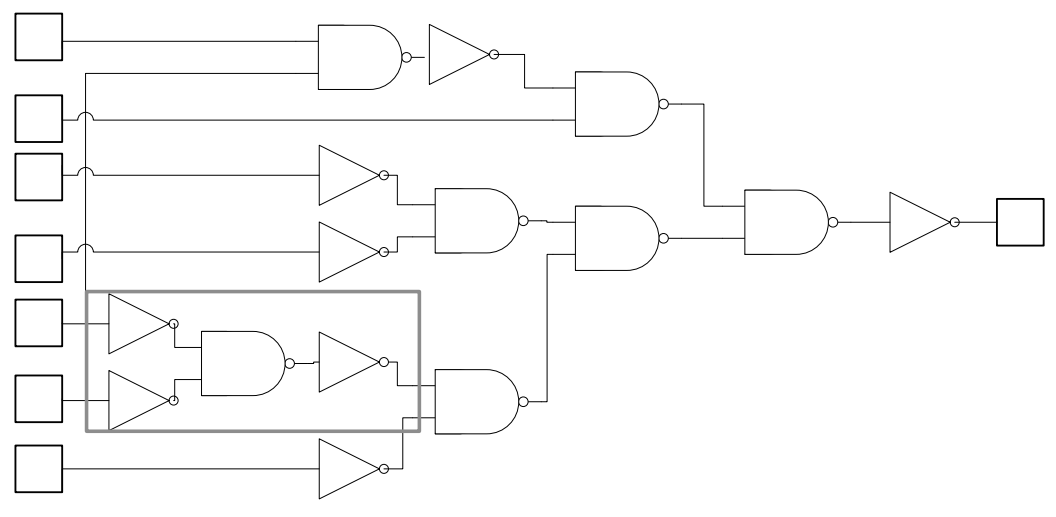
\includegraphics[width=9cm, scale=1]{S4/nor2_pattern.PNG}
    \captionsetup{justification=centering}
    \captionof{figure}{\textit{NOR2} patterns}
\end{minipage}%
\begin{minipage}[t]{0.5\textwidth}
    \centering
    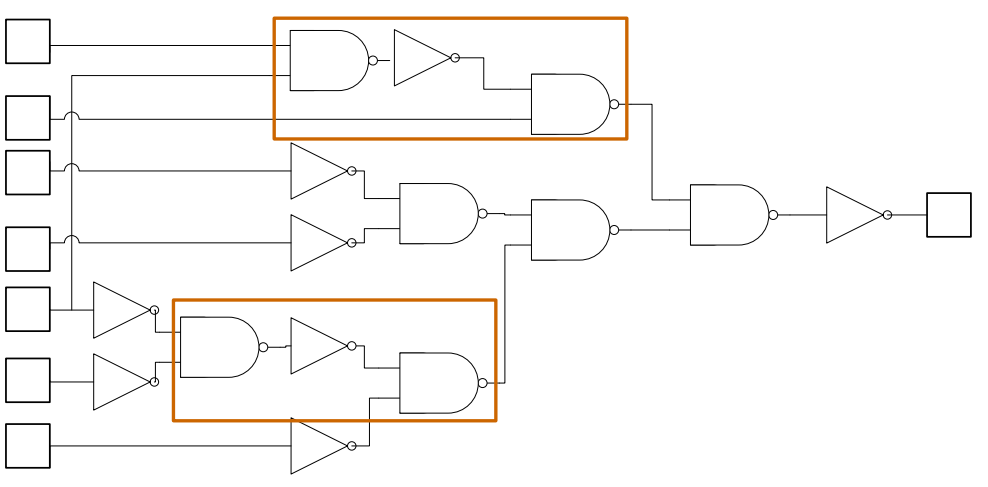
\includegraphics[width=9cm, scale=1]{S4/nand3_pattern.PNG}
    \captionsetup{justification=centering}
    \captionof{figure}{\textit{NAND3} patterns}
\end{minipage}%

\vspace{1cm}
\begin{minipage}[t]{0.5\textwidth}
    \centering
    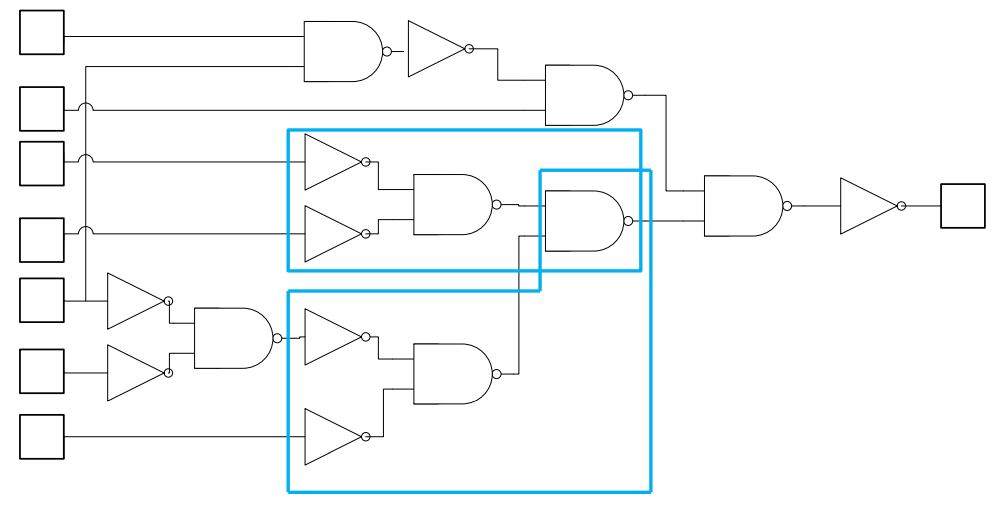
\includegraphics[width=9cm, scale=1]{S4/oai21_pattern.PNG}
    \captionsetup{justification=centering}
    \captionof{figure}{\textit{OAI21} patterns}
\end{minipage}%
\begin{minipage}[t]{0.5\textwidth}
    \centering
    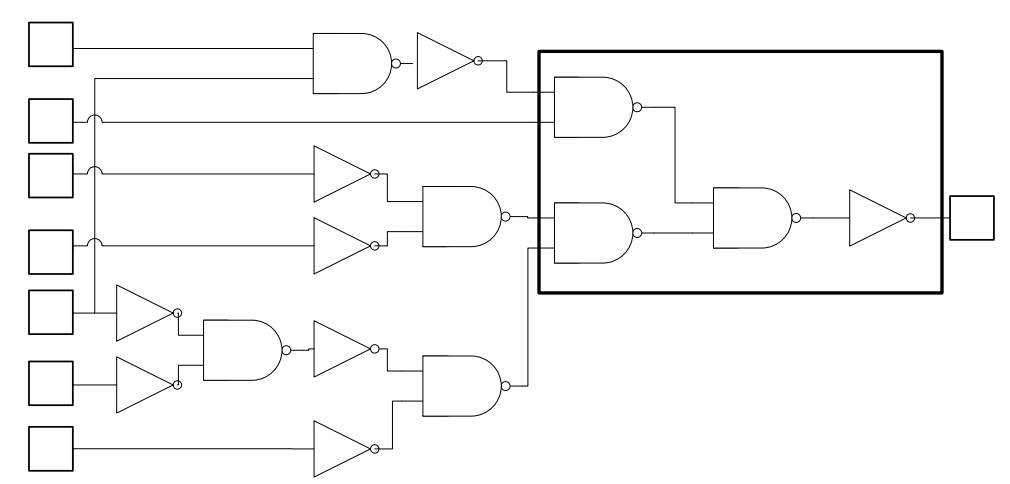
\includegraphics[width=9cm, scale=1]{S4/aoi22_pattern.PNG}
    \captionsetup{justification=centering}
    \captionof{figure}{\textit{AOI22} patterns}
\end{minipage}%

\newpage
\begin{figure}[htp]
    \centering
    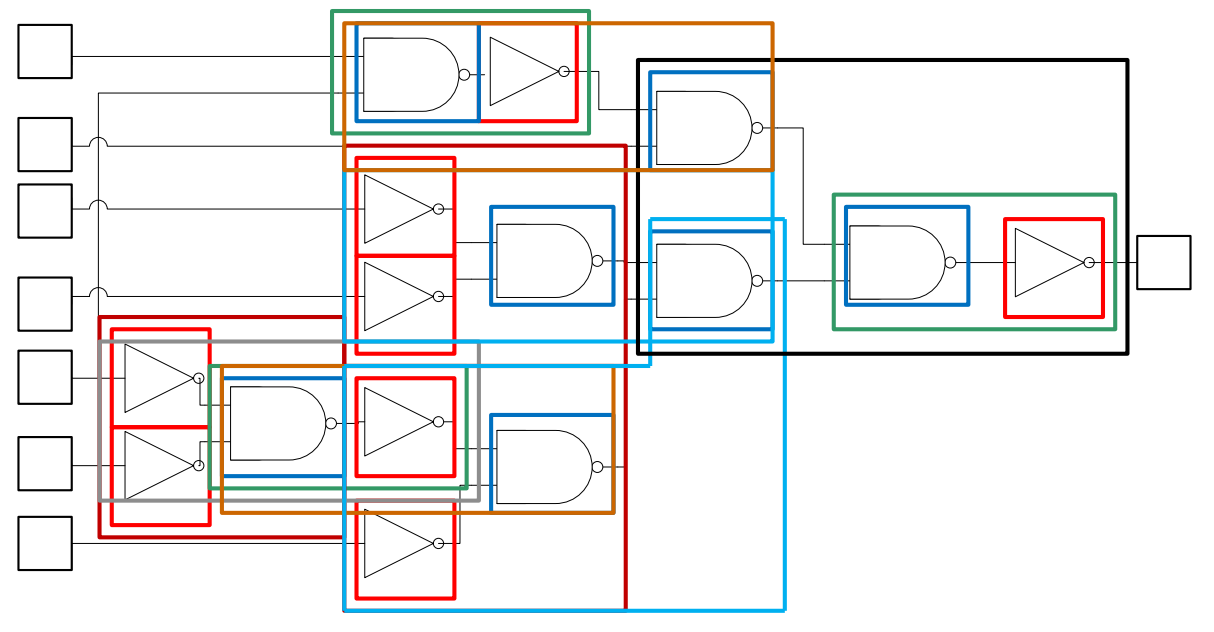
\includegraphics[width=20cm, scale=1]{S4/all_pattern.PNG}
    \caption{All patterns (superimposed)}
\end{figure}

Now the question of \textit{optimal coverage}. Which different combinations shall we use to map the entire network?

\begin{itemize}
    \item Note that a \textit{greedy} approach \textbf{may not be optimal}.
    \item We have to try out all different combinations and see which is optimal. This will be covered later.
\end{itemize}

\subsection{Problems with Structural Matching}
\subsubsection{Structural Matching works on trees only}

\paragraph{Recap: Properties of trees}\mbox{}
\begin{itemize}
    \item Each node in the tree can be connected to many children, but must be connected to \textbf{exactly one parent} (except for the root node).
    \item This constraint means that there are no 'cycles' or 'loops' in the tree
    \item What implications does this have for us?
        \begin{itemize}
            \item Circuits with a \textbf{fan-out} node cannot be represented with a tree
            \item Therefore, we cannot apply \textit{matching} across fan-out nodes!
        \end{itemize}
\end{itemize}

\begin{minipage}[t]{0.5\textwidth}
    \centering
    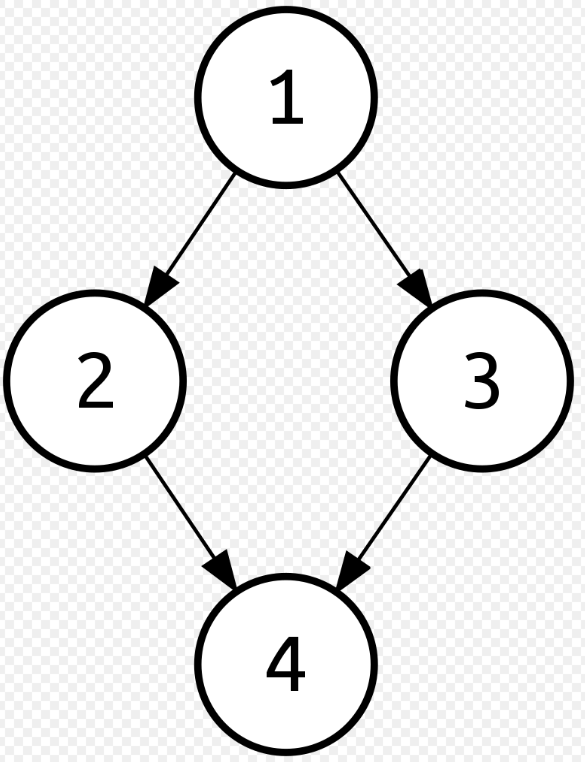
\includegraphics[width=3cm, scale=1]{S4/notATree.PNG}
    \captionsetup{justification=centering}
    \captionof{figure}{Not a tree. Node 4 has more than one parent.}
\end{minipage}%
\begin{minipage}[t]{0.5\textwidth}
    \centering
    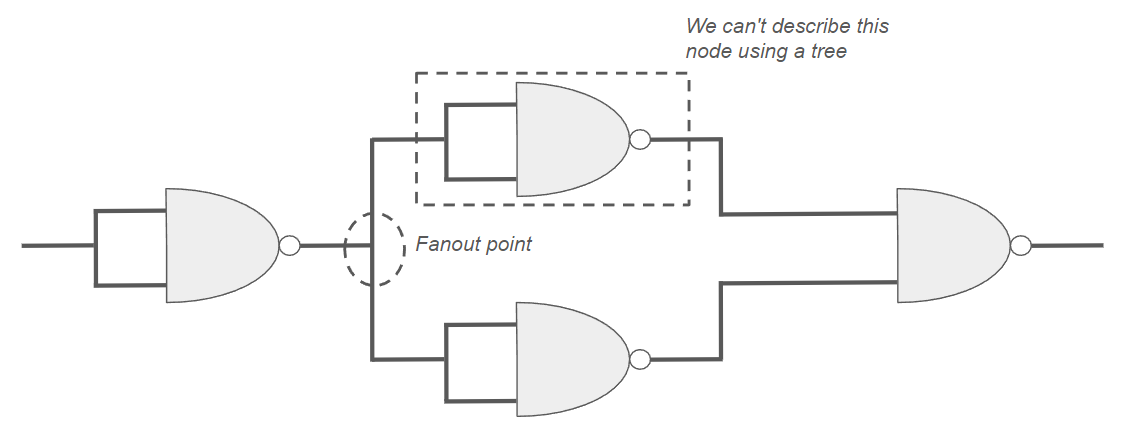
\includegraphics[width=12cm, scale=1]{S4/cantBeDescribed.PNG}
    \captionsetup{justification=centering}
    \captionof{figure}{Circuits with fan-out nodes are an issue}
\end{minipage}%

\vspace{2.5cm}
This means that \textit{XOR} gates cannot be matched, since \textit{XOR} gates require fan-out (by definition)

\begin{figure}[htp]
    \centering
    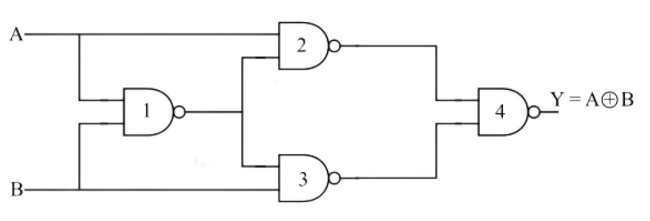
\includegraphics[width=12cm, scale=1]{S4/xorGate.PNG}
    \caption{$A\oplus B = (A \cdot \bar{B}) + (\bar{A} \cdot B)$; Thus \textit{XOR} gates require fan-out}
\end{figure}

\subsubsection{Structural Matching has imperfect matching}
\begin{itemize}
    \item Different structures \textbf{with the same functionality} are not identified by structural matching.
    \item This means that we miss out on potential matches, meaning our final result is not fully optimized
\end{itemize}

\begin{minipage}[t]{0.5\textwidth}
    \centering
    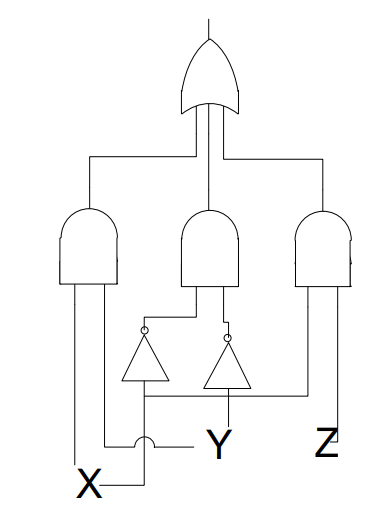
\includegraphics[width=6cm, scale=1]{S4/structural1.PNG}
    \captionsetup{justification=centering}
    \captionof{figure}{$g = xy + \bar{x}\bar{y} + xz$}
\end{minipage}%
\begin{minipage}[t]{0.5\textwidth}
    \centering
    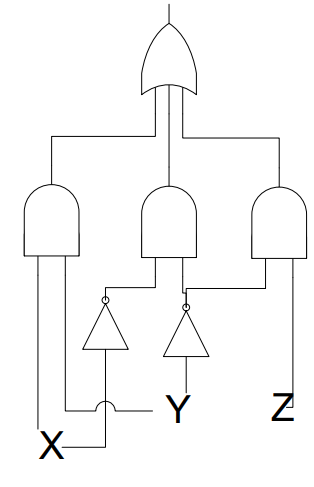
\includegraphics[width=6cm, scale=1]{S4/structural2.PNG}
    \captionsetup{justification=centering}
    \captionof{figure}{$f = xy + \bar{x}\bar{y} + \bar{y}z$}
\end{minipage}%

In the example above, both functions $f$ and $g$ are \textbf{functionally identical} (you can check using truth table), but \textbf{structurally different}.
Structural matching will not identify that they are the same.

The fix to this issue is to do matching by \textit{boolean logic}, rather than by \textit{structure} (ie. isomorphism). This is called \textit{Boolean Matching}.

\newpage
\section{Boolean Matching}
Boolean Matching relies on matching the \textit{pattern} to the \textit{subject} logically

\begin{itemize}
    \item Decomposition independent
    \item Patterns match via \textit{structural match} $\implies$ Patterns match via \textit{boolean match}
        \begin{itemize}
            \item Structurally matched pattern must be logically equivalent
        \end{itemize}
    \item Patterns match via \textit{boolean match} $\centernot \implies$ Patterns match via \textit{structural match}
        \begin{itemize}
            \item Two logically equivalent patterns may have different structures (as we saw in Fig39 and Fig40)
        \end{itemize}
\end{itemize}

\subsection{Boolean Matching - General ideas} 
\begin{enumerate}[label*=\arabic*.]
    \item Define the \textit{cluster function} (what we previously termed \textit{subject graph}) as $f(X) = f(x_{1},x_{2},\dots , x_{n})$; ie. $n$ input variables
    \item Define the \textit{pattern function} (what we previously termed \textit{pattern graph}) as $g(Y) = f(y_{1},y_{2},\dots , y_{m})$; ie. $m$ cell inputs
    \item WLOG, assume $n=m$
    \item Matching of functions $f$ and $g$, involves comparing $f$ and $g$ for \textit{equivalence} (ie. checking if they are logically equivalent)
        \begin{enumerate}[label*=\arabic*.]
            \item Intuitively, we are examining all \textit{permutations} to find valid assignment(s) of variables from \textbf{cluster function} to variables of \textbf{pattern function}
        \end{enumerate}
\end{enumerate}

\begin{figure}[htp]
    \centering
    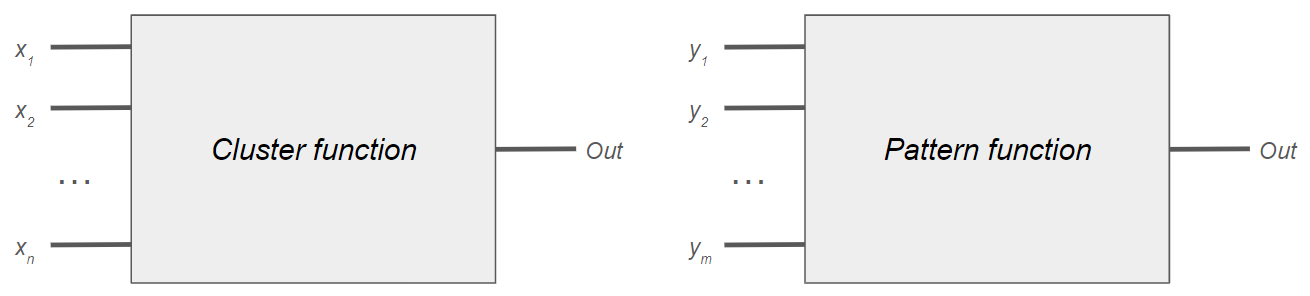
\includegraphics[width=12cm, scale=1]{S5/cluster_pattern_function.PNG}
    \caption{Abstracted view of cluster and pattern functions}
\end{figure}

\begin{minipage}[t]{0.45\textwidth}
    \centering
    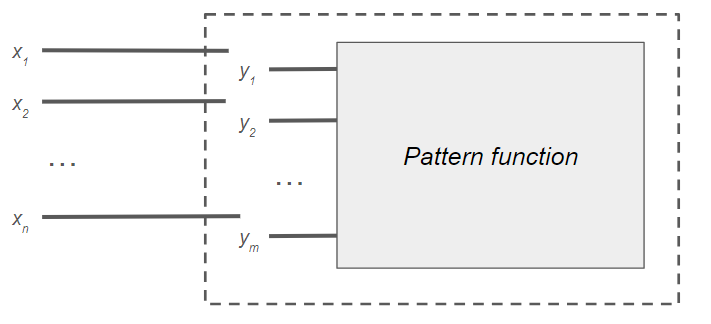
\includegraphics[width=9cm, scale=1]{S5/potentialConnection.PNG}
    \captionsetup{justification=centering}
    \captionof{figure}{There are many different ways (\textit{permutations}) to connect $\{x_{1}, \dots ,x_{n}\}$ with $\{y_{1}, \dots , y_{n}\}$.
                        We need to examine all permutations to find if logical equivalence exists (and if so, under which case is it mapping is it optimal?)}
\end{minipage}%
\begin{minipage}[t]{0.55\textwidth}
    \centering
    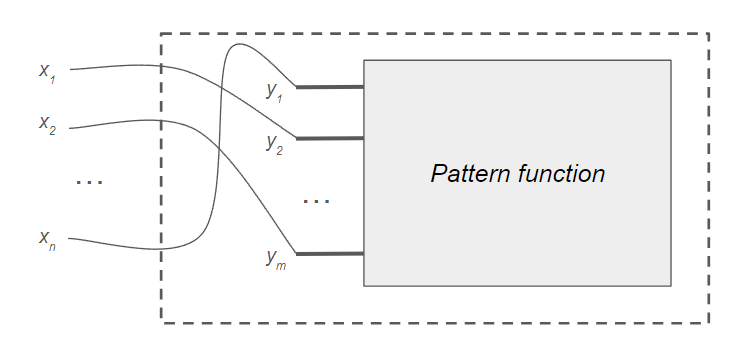
\includegraphics[width=9cm, scale=1]{S5/possibleConnection.PNG}
    \captionsetup{justification=centering}
    \captionof{figure}{One possible connection might be this.\\ Note that $y_{1}$ of pattern function does not correspond to $x_{1}$ of cluster function} 
\end{minipage}%

\newpage
\subsection{Equivalence of functions}
Functions may be logically equivalent under different conditions, let's examine an example.
\subsubsection{Permutation of input variables}
Ordering of input \textit{cluster variables} needs to be changed

\begin{minipage}[c]{0.5\textwidth}
    \centering
    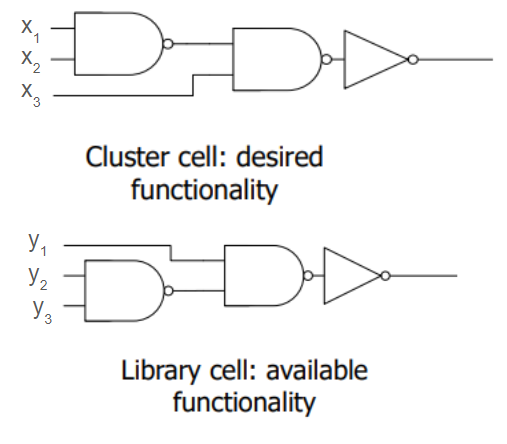
\includegraphics[width=7cm, scale=1]{S5/permute_cluster_library.PNG}
    \captionsetup{justification=centering}
    \captionof{figure}{Can desired functionality be implemented with library cell?}
\end{minipage}%
\begin{minipage}[c]{0.5\textwidth}
    \centering
    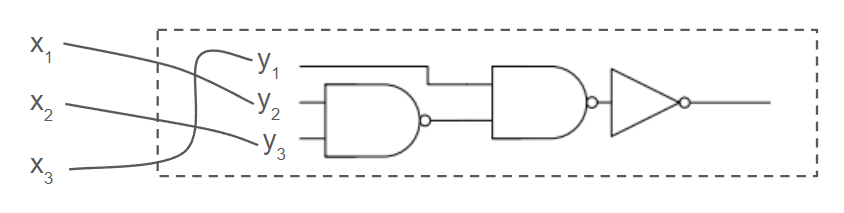
\includegraphics[width=10cm, scale=1]{S5/permutation.PNG}
    \captionsetup{justification=centering}
    \captionof{figure}{One possible permutation that is valid}
\end{minipage}%

\vspace{0.5cm}
Mathematically speaking, we have $g(Y) = f(\rho(X))$ where $\rho$ is some permutation of $X$

For example \dots

\begin{enumerate}[label*=\arabic*.]
    \item Suppose $\Scale[1.25]{f(X) = x_{1}\bar{x_{3}} + x_{2}x_{4}}$
    \item Suppose $\Scale[1.25]{g(Y) = y_{2}\bar{y_{4}} + y_{1}y_{3}}$
    \item $\rho$ reorders $X$ and maps \dots
        \begin{enumerate}[label*=\arabic*.]
            \item $x_{1} \xrightarrow{} y_{2}$
            \item $x_{2} \xrightarrow{} y_{1}$
            \item $x_{3} \xrightarrow{} y_{4}$
            \item $x_{4} \xrightarrow{} y_{3}$
        \end{enumerate}
    \item Hence, $\Scale[1.25]{g(Y) = f(\rho(X))}$
\end{enumerate}

If functions are equivalent when variable order is allowed to change, we term that \textit{P-equivalent}


\subsubsection{Negation of input variables}
Polarity of inputs can be altered, assuming that inputs come from FFs (which provide input and it's complemented version)

\begin{minipage}[c]{0.5\textwidth}
    \centering
    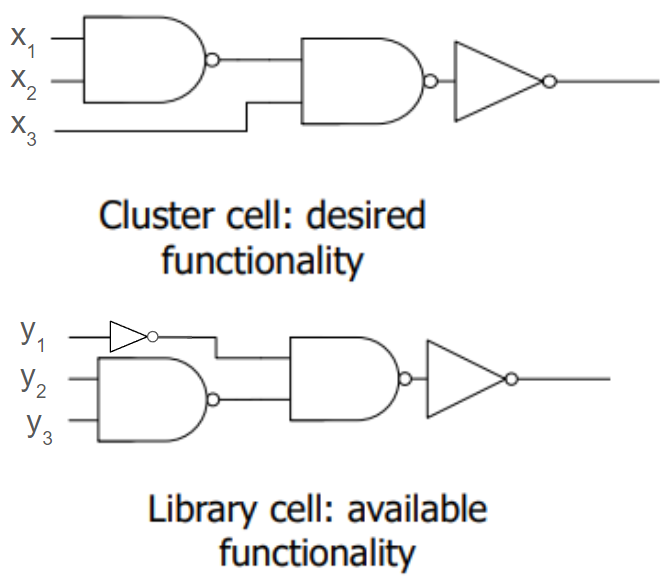
\includegraphics[width=7cm, scale=1]{S5/inputNegate_cluster_library.PNG}
    \captionsetup{justification=centering}
    \captionof{figure}{We cannot directly connect cluster variables to pattern variables now}
\end{minipage}%
\begin{minipage}[c]{0.5\textwidth}
    \centering
    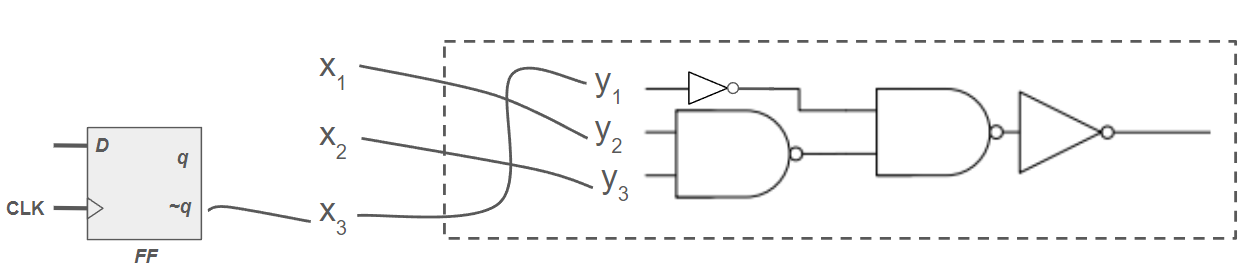
\includegraphics[width=10cm, scale=1]{S5/inputNegation.PNG}
    \captionsetup{justification=centering}
    \captionof{figure}{However, taking $\bar{Q}$ from the input FF solves our problems}
\end{minipage}%

Mathematically speaking, we have $g(Y) = f(\phi(X))$ where $\phi$ maps $x_{i}$ (elements of $X$) either to $y_{i}$ or $\bar{y_{i}}$

For example \dots

\begin{enumerate}[label*=\arabic*.]
    \item Suppose $\Scale[1.25]{f(X) = x_{1} + x_{2} + x_{3}}$
    \item Suppose $\Scale[1.25]{g(Y) = \bar{y_{1}} + \bar{y_{2}} + y_{3}}$
    \item $\phi$ maps \dots
        \begin{enumerate}[label*=\arabic*.]
            \item $x_{1} \xrightarrow{} \bar{y_{1}}$
            \item $x_{2} \xrightarrow{} \bar{y_{2}}$
            \item $x_{3} \xrightarrow{} y_{3}$
        \end{enumerate}
    \item Hence, $\Scale[1.25]{g(Y) = f(\phi(X))}$
\end{enumerate}

If functions are equivalent when polarity of input variable is allowed to change, we term that \textit{N-equivalent}

\subsubsection{Negation of output variables}
Same concept of negation of input variables, but this time at the output

For example \dots

\begin{enumerate}[label*=\arabic*.]
    \item Suppose $\Scale[1.25]{f(X) = x_{1} + x_{2}}$
    \item Suppose $\Scale[1.25]{g(Y) = \bar{y_{1}} \cdot \bar{y_{2}}}$
    \item Do $g(Y) = \bar{f}(X)$
\end{enumerate}

\subsubsection{Summary}
We thus have three categories of equivalence \dots
\begin{itemize}
    \item \textit{NPN-equivalent}: Equivalent under input negation, input permutation, output negation
    \item \textit{PN-equivalent}: Equivalent under input permutation, output negation
    \item \textit{P-equivalent}: Equivalent under input permutation
\end{itemize}

\vspace{0.5cm}
In the \textbf{worst-case} scenario of \textit{NPN-equivalence}, we have to check
($2^{n} \times n! \times 2$) mappings just to determine if logical equivalence exists!
\begin{itemize}
    \item $2^{n}$: $n$ input variables may be negated (either 0 or 1)
    \item $n!$: $n$ input variables have $n!$ different permutations (orderings)
    \item $2$: output variable may be negated (either 0 or 1)
\end{itemize}

That is alot of mappings to consider. \textit{Boolean signatures} give us a way to reduce the number of possibilities.

\section{Boolean Signatures}
Boolean signatures are a compact representation that characterizes \textbf{some} of the properties of a boolean function.

\begin{itemize}
    \item Boolean signatures do not match $\implies$ No match is possible
    \item Boolean signatures match $\implies$ Match \textbf{may} be possible
        \begin{itemize}
            \item Each boolean function has a \textbf{unique} signature, but a signature can be related to $>1$ functions (this problem is termed \textit{aliasing})
            \item Therefore, signature matching is \textit{necessary}, but \textbf{not} a \textit{sufficient} condition
            \item Only if \textbf{all} possible boolean signatures match, then we can say that  function match is possible  (but this is not a practical way to do so)
        \end{itemize}
\end{itemize}

Therefore, the main idea is to use some simple boolean signatures to filter out the solution space, before we start checking function equivalence.
If we know that some functions already have non-matching boolean signatures, we need not consider them during the function equivalence stage.

Note that whether the boolean signatures match, also depends on equivalence type we are checking for (NPN, PN, P)?

\newpage
\subsection{Example of boolean signatures}
\subsubsection{Function symmetry}
How many sets of variables are pairwise interchangable without affecting the logic?
\begin{itemize}
    \item $\Scale[1.25]{\bar{A}\bar{B} + ABC}$; $A,B$ are pairwise interchangable (1 set)
    \item $\Scale[1.25]{\bar{B}(A + \bar{C}) + C}$; No variables are pairwise interchangable (0 set)
\end{itemize}

\subsubsection{Number of unate/binate variables}
\begin{itemize}
    \item Unate variables: Variables with which a function \textit{monotonically} increases/decreases
    \item Binate variables: Not unate variables 
\end{itemize}

An example \dots
$A\bar{C} + \bar{A}B$
\begin{itemize}
    \item $B,C$ are unate variables (B \textbf{always} pulls towards logic high, C \textbf{always} pulls towards logic low)
    \item $A$ is binate variable (A can pull to logic high or low, depending on circumstances)
\end{itemize}

\subsection{Summary}
\begin{figure}[htp]
    \centering
    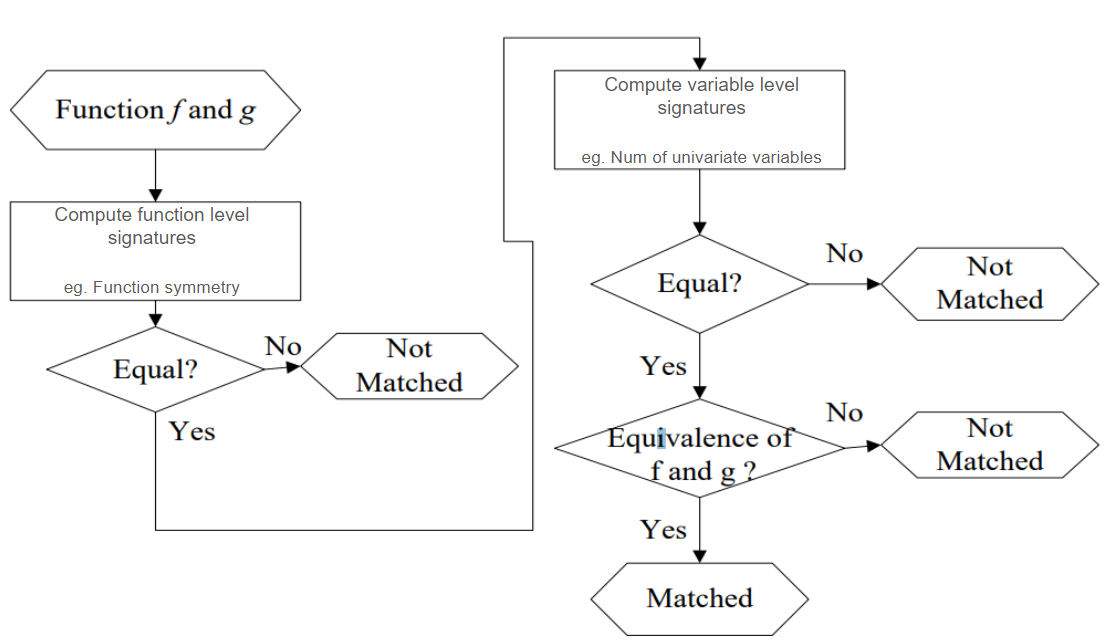
\includegraphics[width=15cm, scale=1]{S5/signatureFlow.PNG}
    \caption{Flowchart}
\end{figure}

\section{Covering}
Once we find matches between the pattern-tree (decomposed library cells) and subgraphs of the subject tree, which match shall we pick to implement our actual circuit?

Formally speaking \dots
\begin{itemize}
    \item Define \textit{covering} as a collection of pattern graphs st. every node of the subject graph is contained in one (or more) of the pattern graphs
    \item We then want to find the \textbf{minimum} cost covering - which particular collection of pattern graphs will achieve this?
\end{itemize}

\subsection{Covering of trees and DAGs}
\subsubsection{Trees}

\begin{minipage}[c]{0.5\textwidth}
    \centering
    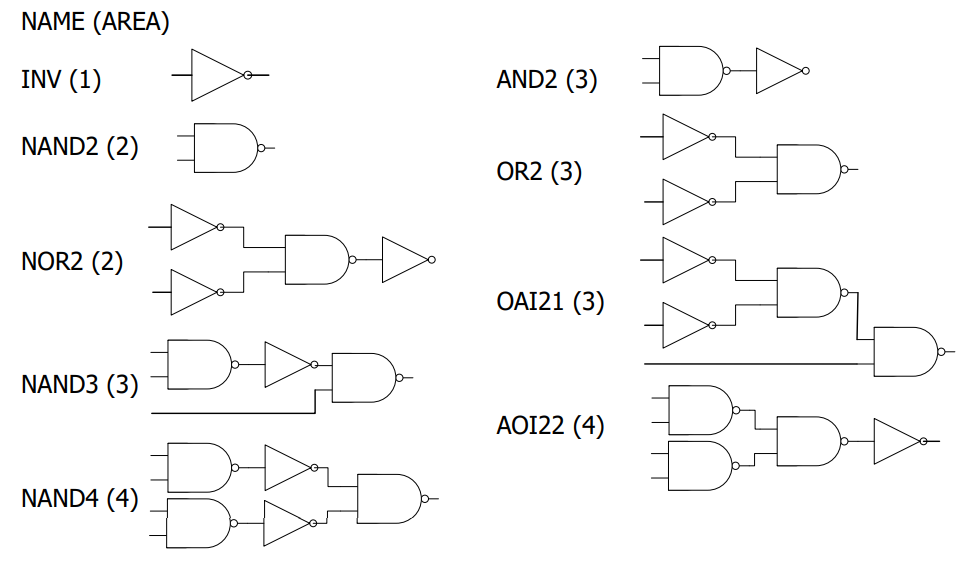
\includegraphics[width=7cm, scale=1]{S4/pattern_library.PNG}
    \captionsetup{justification=centering}
    \captionof{figure}{Cell Library}
\end{minipage}%
\begin{minipage}[c]{0.5\textwidth}
    \centering
    \includegraphics[width=10cm, scale=1]{S6/subject_noFanOut.PNG}
    \captionsetup{justification=centering}
    \captionof{figure}{Subject graph \textbf{with no fanout nodes}}
\end{minipage}%

\begin{itemize}
    \item Consider the example above, where the subject graph \textbf{has no fanout nodes}.
    \item We know that we can convert the subject graph to a \textit{tree}, since there are no fan-out nodes
    \item We also know that we can covert the cell library to it's appropriate tree representation
    \item Therefore, the covering problem to cover the 'subject-tree' using 'pattern-trees', which \textbf{has a P solution}.
\end{itemize}

\begin{minipage}[c]{0.5\textwidth}
    \centering
    \includegraphics[width=9cm, scale=1]{S6/trivialCovering.PNG}
    \captionsetup{justification=centering}
    \captionof{figure}{Trivial covering}
\end{minipage}%
\begin{minipage}[c]{0.5\textwidth}
    \centering
    \includegraphics[width=9cm, scale=1]{S6/betterCovering.PNG}
    \captionsetup{justification=centering}
    \captionof{figure}{Better covering}
\end{minipage}%

\begin{figure}[htp]
    \centering
    \includegraphics[width=12cm, scale=1]{S6/evenBetter.PNG}
    \caption{Even better covering}
\end{figure}

\newpage
\subsubsection{DAGs}

\begin{minipage}[c]{0.5\textwidth}
    \centering
    \includegraphics[width=11cm, scale=1]{S4/xorGate.PNG}
    \captionsetup{justification=centering}
    \captionof{figure}{\textit{XOR} gate}
\end{minipage}%
\begin{minipage}[c]{0.5\textwidth}
    \centering
    \includegraphics[width=6cm, scale=1]{S6/xor_dag.PNG}
    \captionsetup{justification=centering}
    \captionof{figure}{\textit{XOR} gate representation - DAG}
\end{minipage}%

\vspace{0.5cm}
Covering a 'subject-\textbf{DAG}' using a 'pattern-tree' is termed \textit{DAG-covering}, and is \textbf{NP-hard}.

\paragraph{Treeifying}\mbox{}\\
Partioning a circuit with fan-out nodes (ie. DAG) at the fan-out node points, thereby forming a collection of \textbf{trees}.

\begin{figure}[htp]
    \centering
    \includegraphics[width=12cm, scale=1]{S3/partitionedGraph.PNG}
    \caption{DAG is now transformed into a collection of subnetworks, where each subnetwork is a tree}
\end{figure}

\begin{itemize}
    \item We can then use $P$ solution of tree-covering on each of these sub-networks.
    \item The tradeoff is lowered optimization - We are not able to do inter-subnetwork optimizations
\end{itemize}

\vspace{0.5cm}
Also note that when the DAG is broken into trees at the fan-out points, some of the logic is duplicated.

\begin{minipage}[t]{0.5\textwidth}
    \centering
    \includegraphics[width=9cm, scale=1]{S6/fanout.PNG}
    \captionsetup{justification=centering}
    \captionof{figure}{DAG\\($\exists$ route between leaf(input) to \textbf{two} roots(outputs))}
\end{minipage}%
\begin{minipage}[t]{0.5\textwidth}
    \centering
    \includegraphics[width=10cm, scale=1]{S6/brokenDAG.PNG}
    \captionof{figure}{Logic at fan-out node is duplicated}
\end{minipage}%

\newpage
\subsection{Optimal tree covering using Dynamic Programming}
\begin{itemize}
    \item We use the \textit{memoization} DP approach, visiting the subject tree \textbf{bottom-up} (it's easier this way)
    \item At each vertex, we attempt to match the \textbf{locally} rooted sub-tree to all library cells
        \begin{itemize}
            \item Find the best match and record it at the vertex (ie. Memoization)
        \end{itemize}
    \item Work your way up to the root
\end{itemize}

\subsubsection{DP example}

\begin{figure}[htp]
    \centering
    \includegraphics[width=12cm, scale=1]{S6/dp_start.PNG}
    \caption{Subject and Pattern trees}
\end{figure}

\begin{figure}[htp]
    \centering
    \includegraphics[width=12cm, scale=1]{S6/dp.PNG}
    \caption{Optimally cover the Subject tree using Pattern trees\\
                Approach this using DP (Memoization)}
\end{figure}

\newpage
\section{Technology Mapping on FPGAs}
For FPGAs, the library cells are \textit{LUTs} (higher abstraction level than ASICs).

\subsection{How to do matching with LUTs?}
Unlike previous sections, we do not decompose CLBs (library cell of FPGAs) using primitives (eg. \textit{NAND2} and \textit{INV}) and try to match using them, as it is not practical.
For example, a 4-input LUT can implement $2^{2^{4}} = 256$ possible combinational functions. Decomposing all 256 of those combinational functions is not a good idea.

So how do we match with LUTs? We simply configure the \textit{LUT-mask} to match the output of the cluster function.

\subsubsection{LUT Matching - Example}
Suppose we want to match a \textit{NAND}-gate with a \textit{4LUT}.

\begin{figure}[htp]
    \centering
    \includegraphics[width=8cm, scale=1]{S7/nandTruth.PNG}
    \caption{\textit{NAND} truth table}
\end{figure}

We derive the truth table for a \textit{4LUT} that matches the \textit{NAND}'s truth table, and simply 'copy' $y$ over to the \textit{LUT-mask}.

\begin{minipage}[c]{0.5\textwidth}
    \centering
    \includegraphics[width=3cm, scale=1]{S7/lutTruth1.PNG}
    \captionof{figure}{Notice that $x_{3}$ and $x_{4}$ inputs are 'useless'}
\end{minipage}%
\begin{minipage}[c]{0.5\textwidth}
    \centering
    \includegraphics[width=8cm, scale=1]{S7/lutmask.PNG}
    \captionof{figure}{LUT-mask of 4LUT}
\end{minipage}%

We can see that it is very inefficient (in terms of hardware resources) to match the \textit{NAND}-gate with a \textit{4LUT}.

\newpage
\subsection{Mapping and Covering on FPGAs}
Simply put, FPGA mapping involves transforming the original \textit{subject} network into another network,
where \textbf{every} node corresponds to an \textit{nLUT} (where \textit{nLUT} is the one afforded by our library cell).

Covering is then finding the optimal mapping to utilize, suject to some constraints (ie. use the minimal number of LUTs possible).

Assume that we have decomposed our subject network using whatever primitives were available. Below is how we would do FPGA mapping and covering \dots

\begin{figure}[htp]
    \centering
    \includegraphics[width=12cm, scale=1]{S7/fpgaMapping.PNG}
    \captionsetup{justification=centering}
    \caption{We require 3 \textit{5LUT}s or 6 \textit{3LUT}s to map \& cover this circuit\\
                Notice that a \textit{5LUT} can implement a \textit{4LUT}, one of the inputs will just be 'X'}
\end{figure}

\subsection{Bin Packing}
\begin{itemize}
    \item So far, all our SOP expressions can each 'fit' into a single LUT, but this is not always the case.
    \item Consider an SOP expression of a single-output function, suppose it has at most $n$ variables
        \begin{itemize}
            \item If we have an $nLUT$, then the \textbf{entire} SOP expression can be implemented by one $nLUT$ (which is what we previously assumed)
        \end{itemize}
    \item Suppose this SOP expression has $> n$ variables now
        \begin{itemize}
            \item If we only have an $nLUT$, then the SOP expression needs to be 'split' up and assigned to different $nLUT$s
            \item This ideas is similar (but not quite identical) to the \textit{bin packing problem}, where we must pack a given set of objects (here product terms) of bounded size into bins (here tables)
        \end{itemize}
    \item It is not exactly similar to the \textit{bin packing problem}, since partitioning alone is not sufficient. We require \textbf{more bins} to hold the combined partitioned terms
        \begin{itemize}
            \item Suppose \textit{table size} is $n = 3$ (ie. It's a \textit{3LUT})
            \item Suppose \textit{SOP expression} is $f = ab + cd$
            \item 2 \textit{3LUT}s are needed to implement $ab$ and $cd$, but 1 more \textit{3LUT} is needed to combine them together
            \item Notice that there is room for optimization. For each \textit{3LUT}, one of the inputs is unused. Could we squeeze additional logic into there? This leads us to \textit{Modified Bin Packing}.
        \end{itemize}
\end{itemize}

\subsubsection{Modified Bin Packing (Heuristic algorithm)}
\begin{itemize}
    \item Iterate the following steps until all product terms have been 'binned'
        \begin{enumerate}
            \item Select product term with the most variables
            \item Place it into any table where it fits
            \item If no table has enough place to fit it, create a new table and place it there
        \end{enumerate}
    \item When all product terms are 'binned', do the following steps
        \begin{enumerate}
            \item Find the table $t_{i}$ with the fewest number of \textbf{unused} variables (alternatively, table with most number of \textbf{used} variables) and associate a variable $v_{i}$ with it's \textbf{output}
            \item Assign $v_{i}$ to the first table $t_{j}$ that can accept it
            \item Repeat from (1) until only one table is left
        \end{enumerate}
\end{itemize}

\paragraph{Modified Bin Packing - Example}\mbox{}
\begin{itemize}
    \item Suppose \textit{table size} is $n = 3$ (ie. It's a \textit{3LUT})
    \item Suppose \textit{SOP expression} is $f = ab + cd$
\end{itemize}

\vspace{0.3cm}
\begin{enumerate}[label*=\arabic*.]
    \item One table is created for $ab$, call it $t_{1}$
    \item $cd$ cannot fit in $t_{1}$, create another table $t_{2}$ for it
    \item All terms finished. Let's pick $t_{1}$ as the table with fewest number of unused variables
    \item Associate variable $v_{1}$ with $t_{1}$ (representing the table's output)
    \item Fit $v_{1}$ into the unused \textbf{input} of $t_{2}$
    \item Terminate algorithm, only one table ($t_{2}$) left
    \item Final output of is $f = v_{1} + cd$, which can be implemented by 2 \textit{3LUT}s, compared to 3 \textit{3LUT}s before
\end{enumerate}

\begin{figure}[htp]
    \centering
    \includegraphics[width=8cm, scale=1]{S7/binPacked.PNG}
    \caption{Modified Bin Packing}
\end{figure}

\subsection{CLB packing}
Usually, the CLB's in the FPGAs have more than a singe LUT within them.

\begin{figure}[htp]
    \centering
    \includegraphics[width=12cm, scale=1]{S7/logicBlock.PNG}
    \captionsetup{justification=centering}
    \caption{Logic Block\\
                Observe that the LUTs can share inputs as well}
\end{figure}

\textit{Logic block packing} packs several LUTs and registers into one logic block under the following constraints
\begin{itemize}
    \item Number of LUTs in a logic block
    \item Number of \textbf{distinct} input signals
\end{itemize}

\newpage
Therefore, our optimization goal is to \dots
\begin{itemize}
    \item Pack LUTs st. routing signals are \textbf{minimized} between logic blocks
        \begin{itemize}
            \item External routing is expensive, internal routing within the logic block is cheaper
        \end{itemize}
    \item Fill each logic block to it's maximal capacity, to reduce to total number of logic blocks in the FPGA fabric
\end{itemize}

We can apply the same ideas of 'bin-packing' as covered in the previous sections.

\subsection{Summary}
Technology mapping on FPGAs involves \dots
\begin{itemize}
    \item Mapping
    \item Covering
    \item \textbf{Packing}
\end{itemize}


\end{document}